\providecommand{\main}{../../../..}
\documentclass[\main/dresen_thesis.tex]{subfiles}
\begin{document}
  \label{sec:looselyPackedNS:bilayerStacks:pnr}
  \begin{figure}[tb]
    \centering
    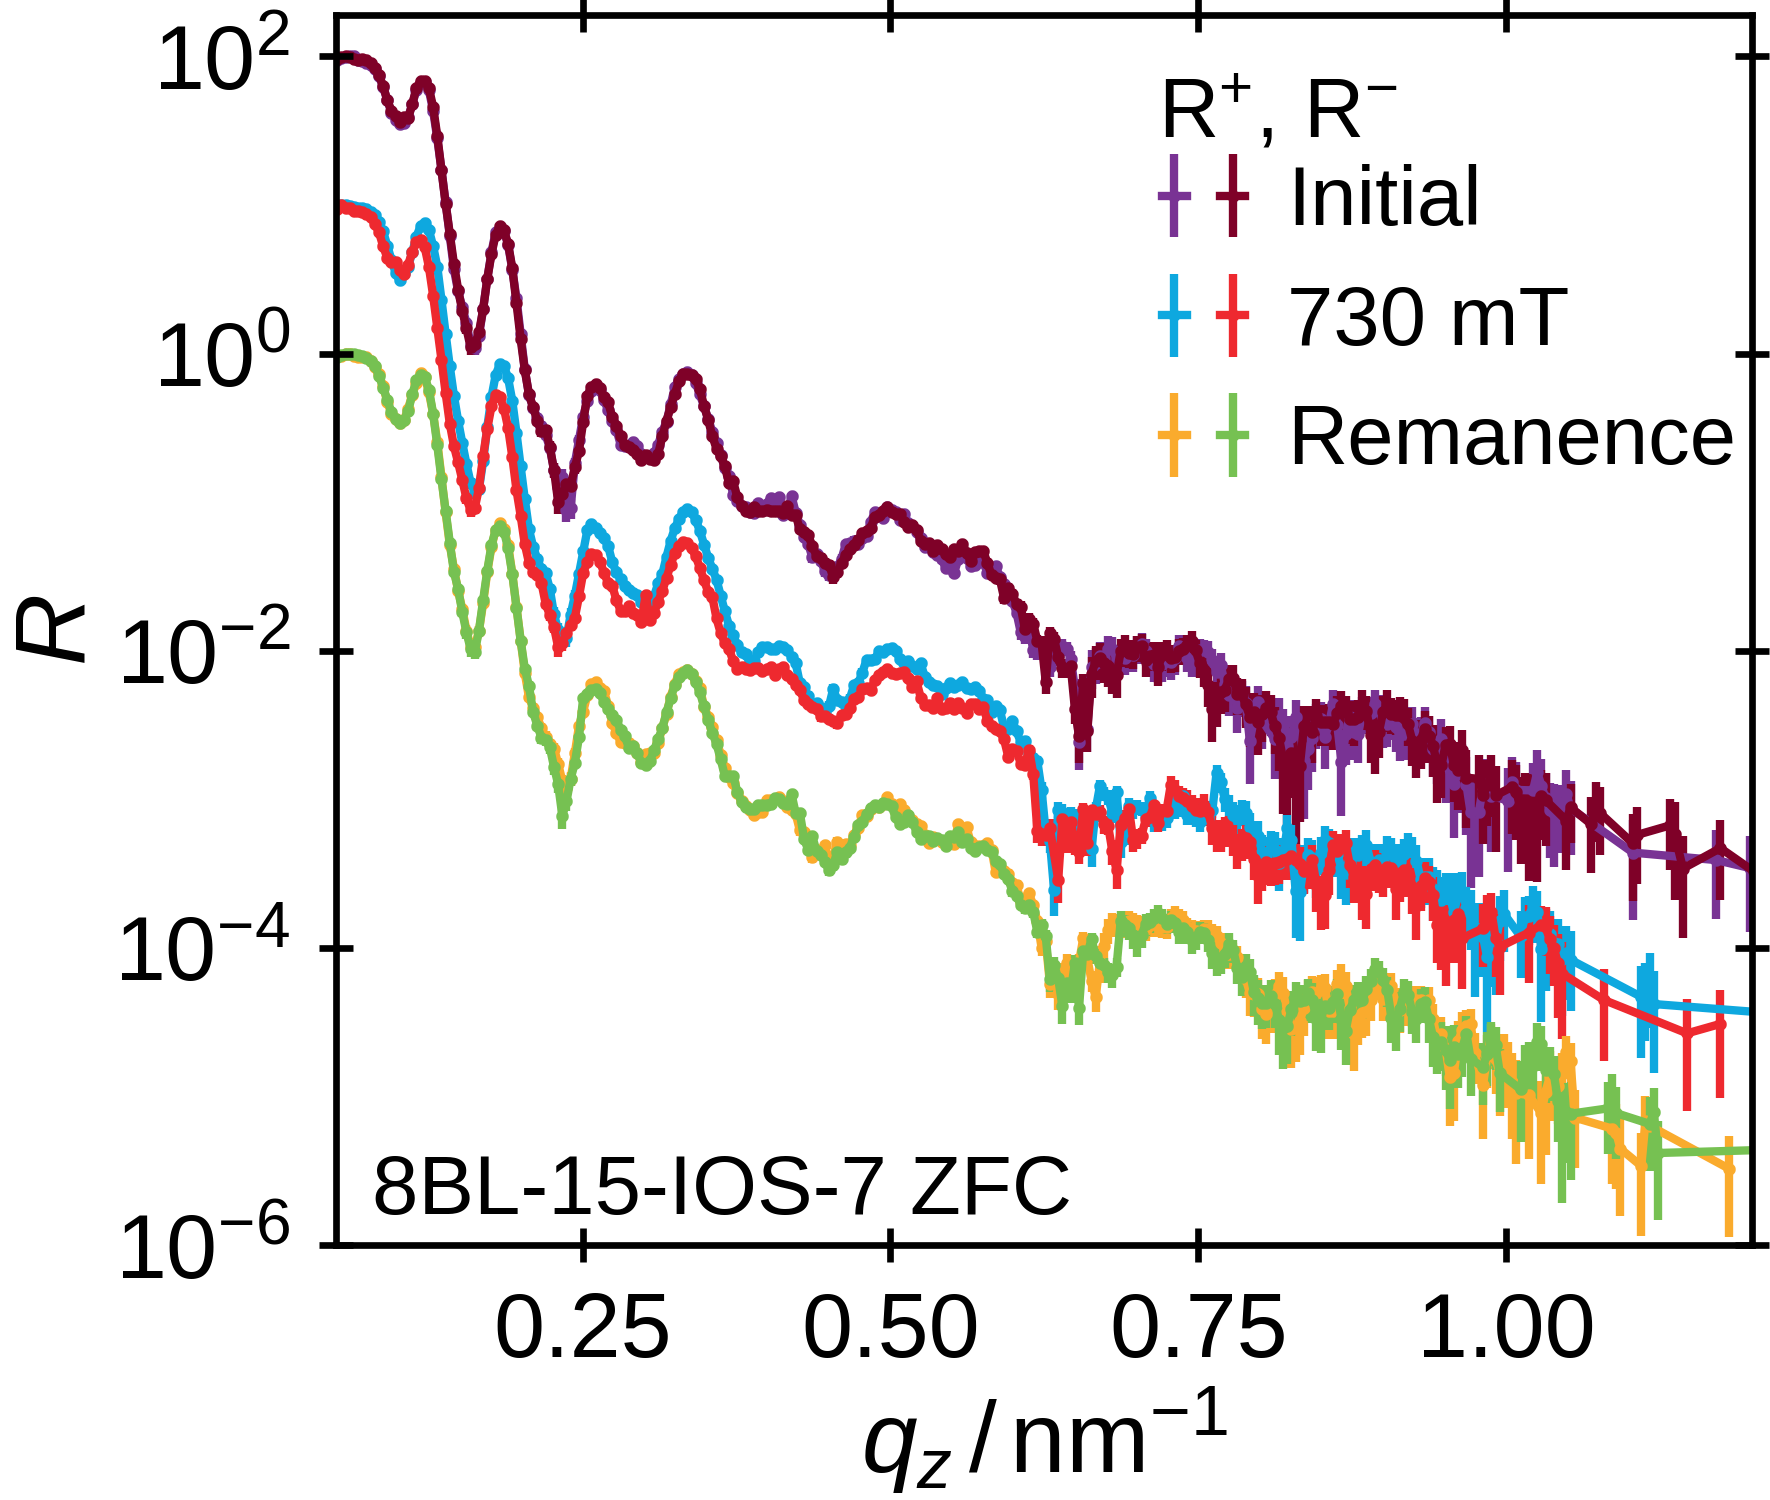
\includegraphics{looselyPackedNP_VerticalStructure_8BL-15-IOS-7_PNR_ZFC30K}
    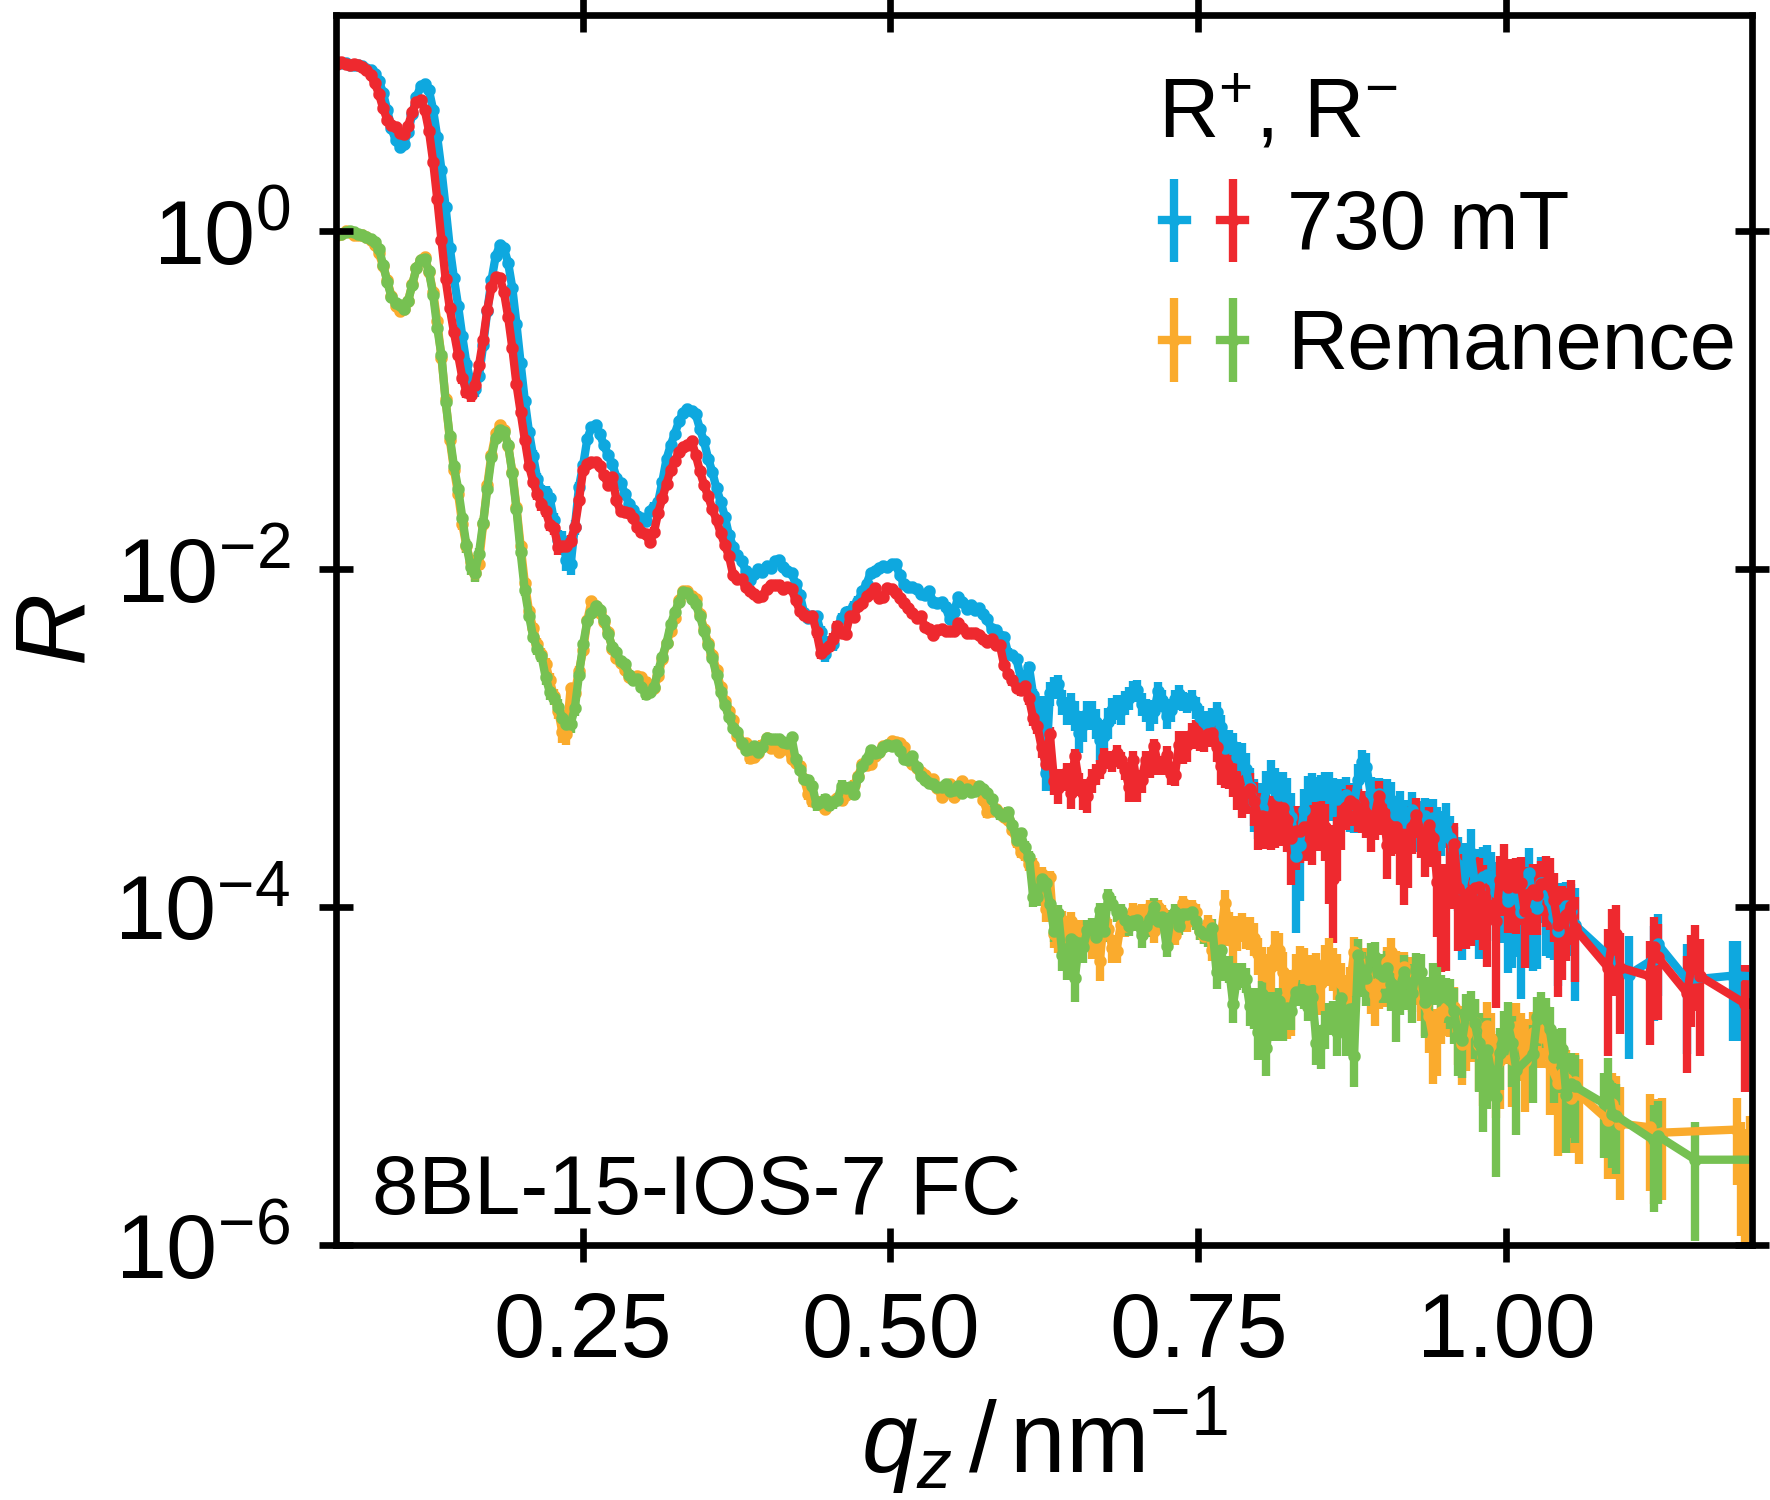
\includegraphics{looselyPackedNP_VerticalStructure_8BL-15-IOS-7_PNR_FC30K}
    \caption{\label{fig:looselyPackedNP:bilayer:pnr:8BL-15-IOS7}X-ray reflectometry from SC-IOS-11 (left) and SC-IOS-7 (right). The inset shows the scattering length density model of the fitted reflectometry curve (black).}
  \end{figure}

  \begin{figure}[tb]
    \centering
    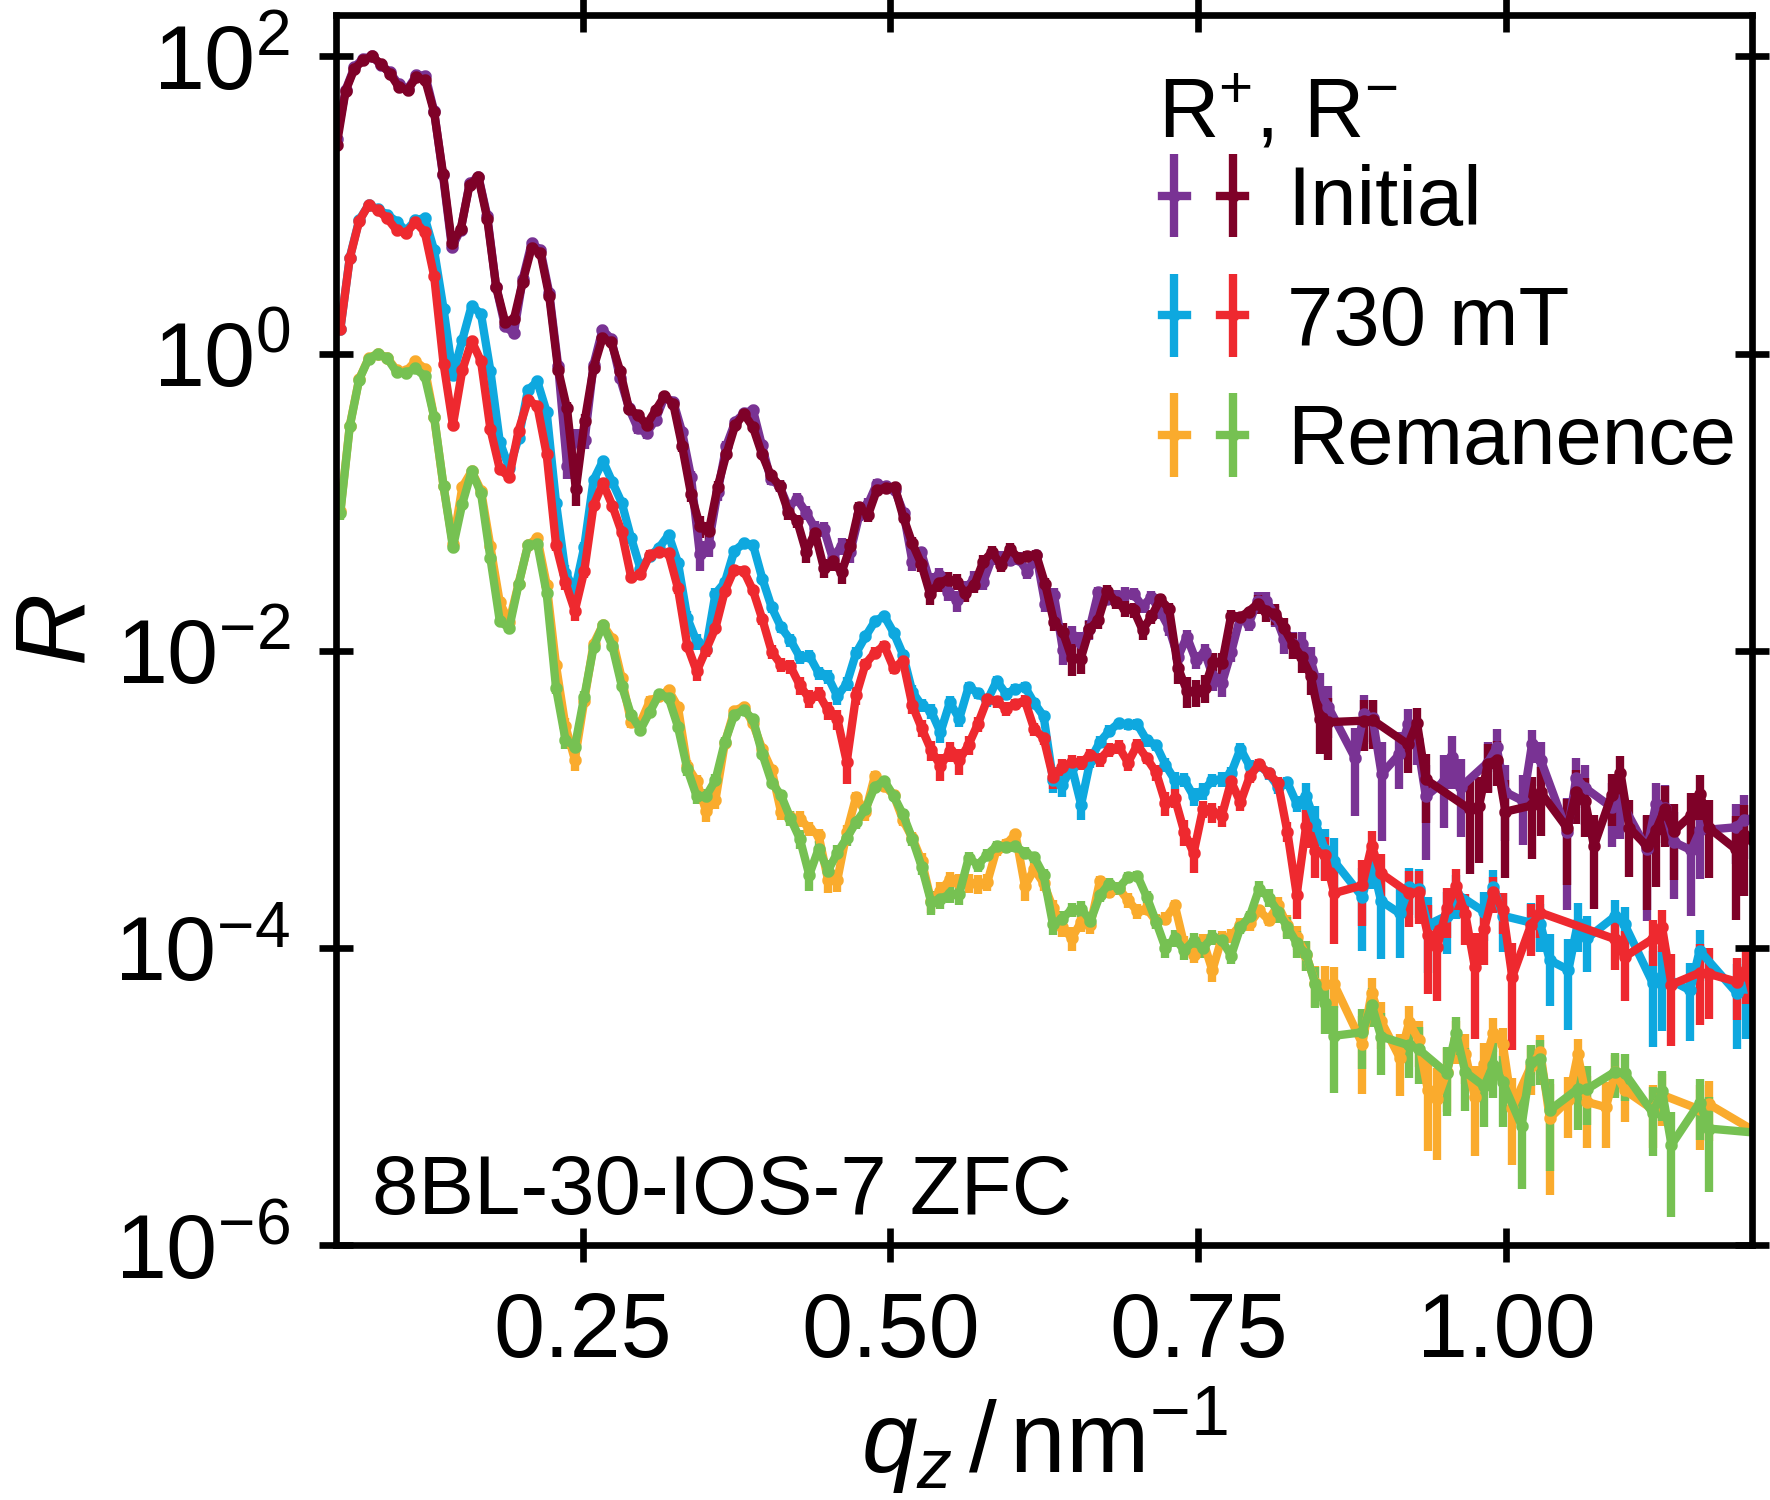
\includegraphics{looselyPackedNP_VerticalStructure_8BL-30-IOS-7_PNR_ZFC30K}
    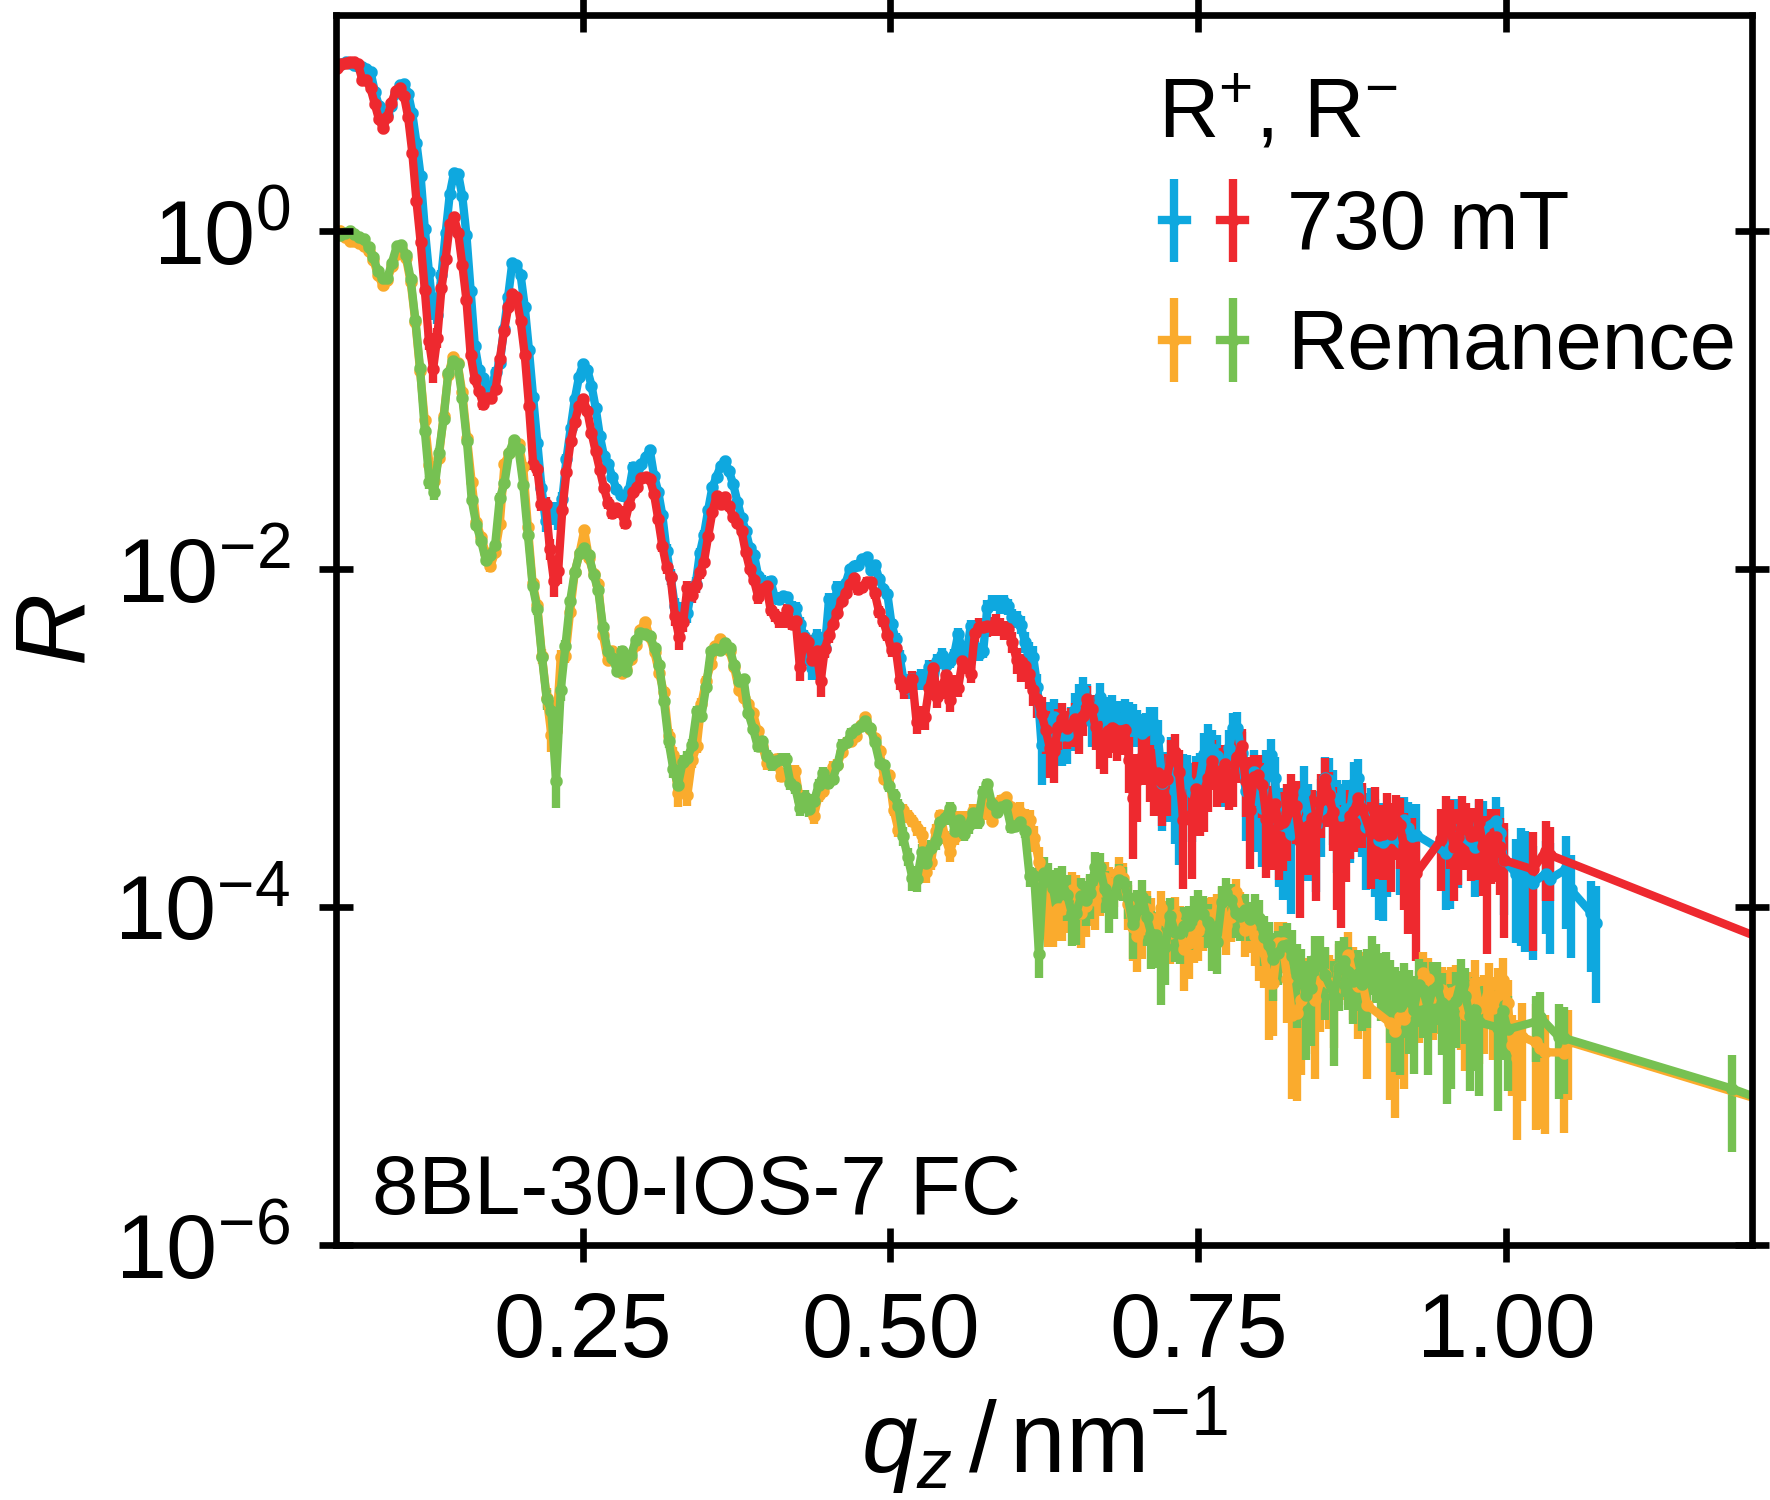
\includegraphics{looselyPackedNP_VerticalStructure_8BL-30-IOS-7_PNR_FC30K}
    \caption{\label{fig:looselyPackedNP:bilayer:pnr:8BL-15-IOS7}X-ray reflectometry from SC-IOS-11 (left) and SC-IOS-7 (right). The inset shows the scattering length density model of the fitted reflectometry curve (black).}
  \end{figure}

  \begin{figure}[tb]
    \centering
    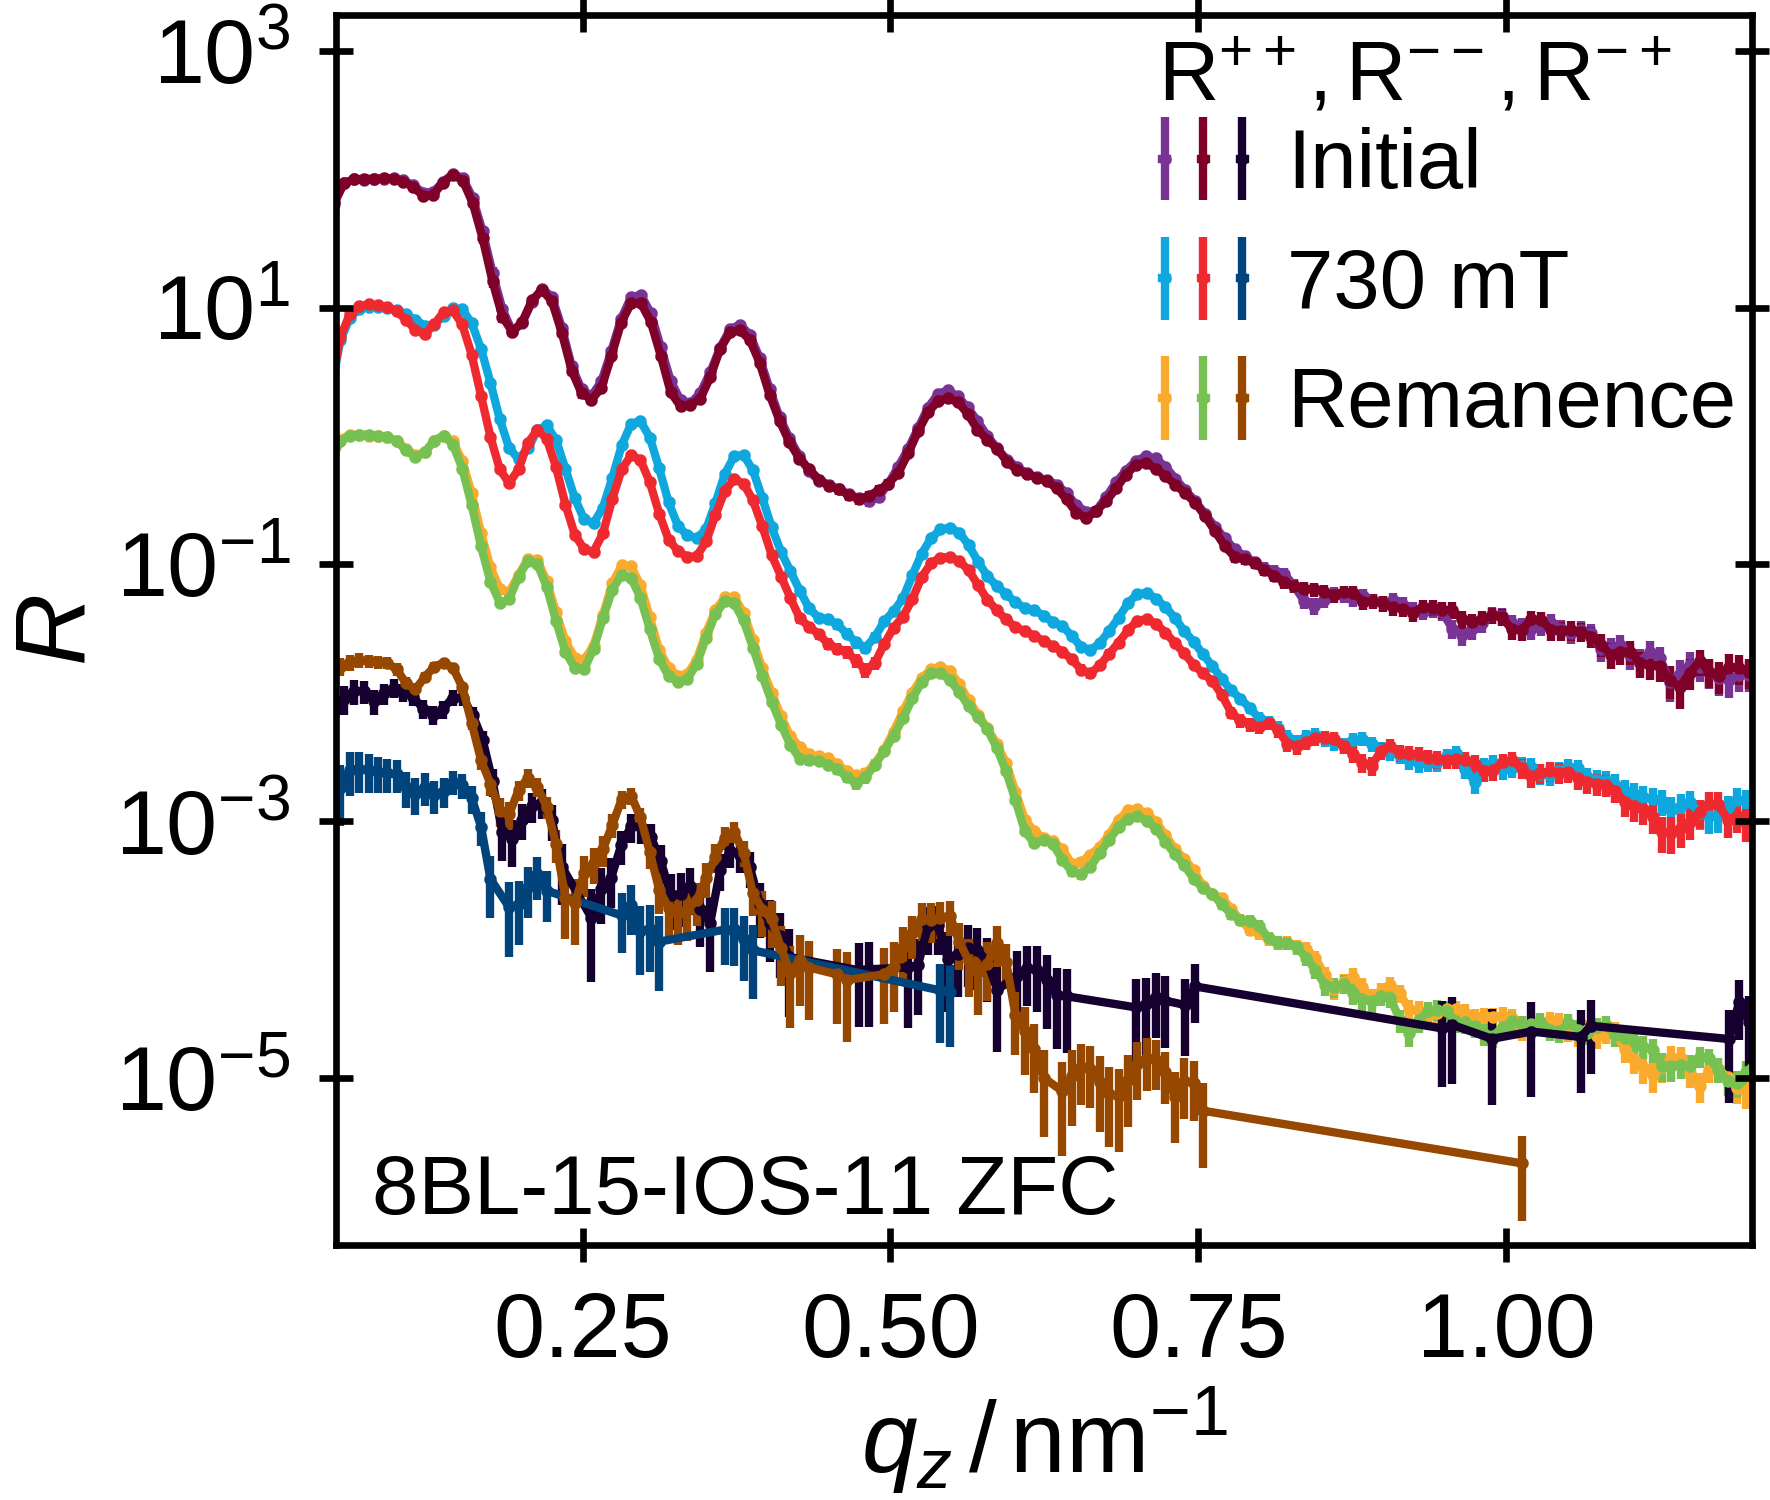
\includegraphics{looselyPackedNP_VerticalStructure_8BL-15-IOS-11_PNR_ZFC30K}
    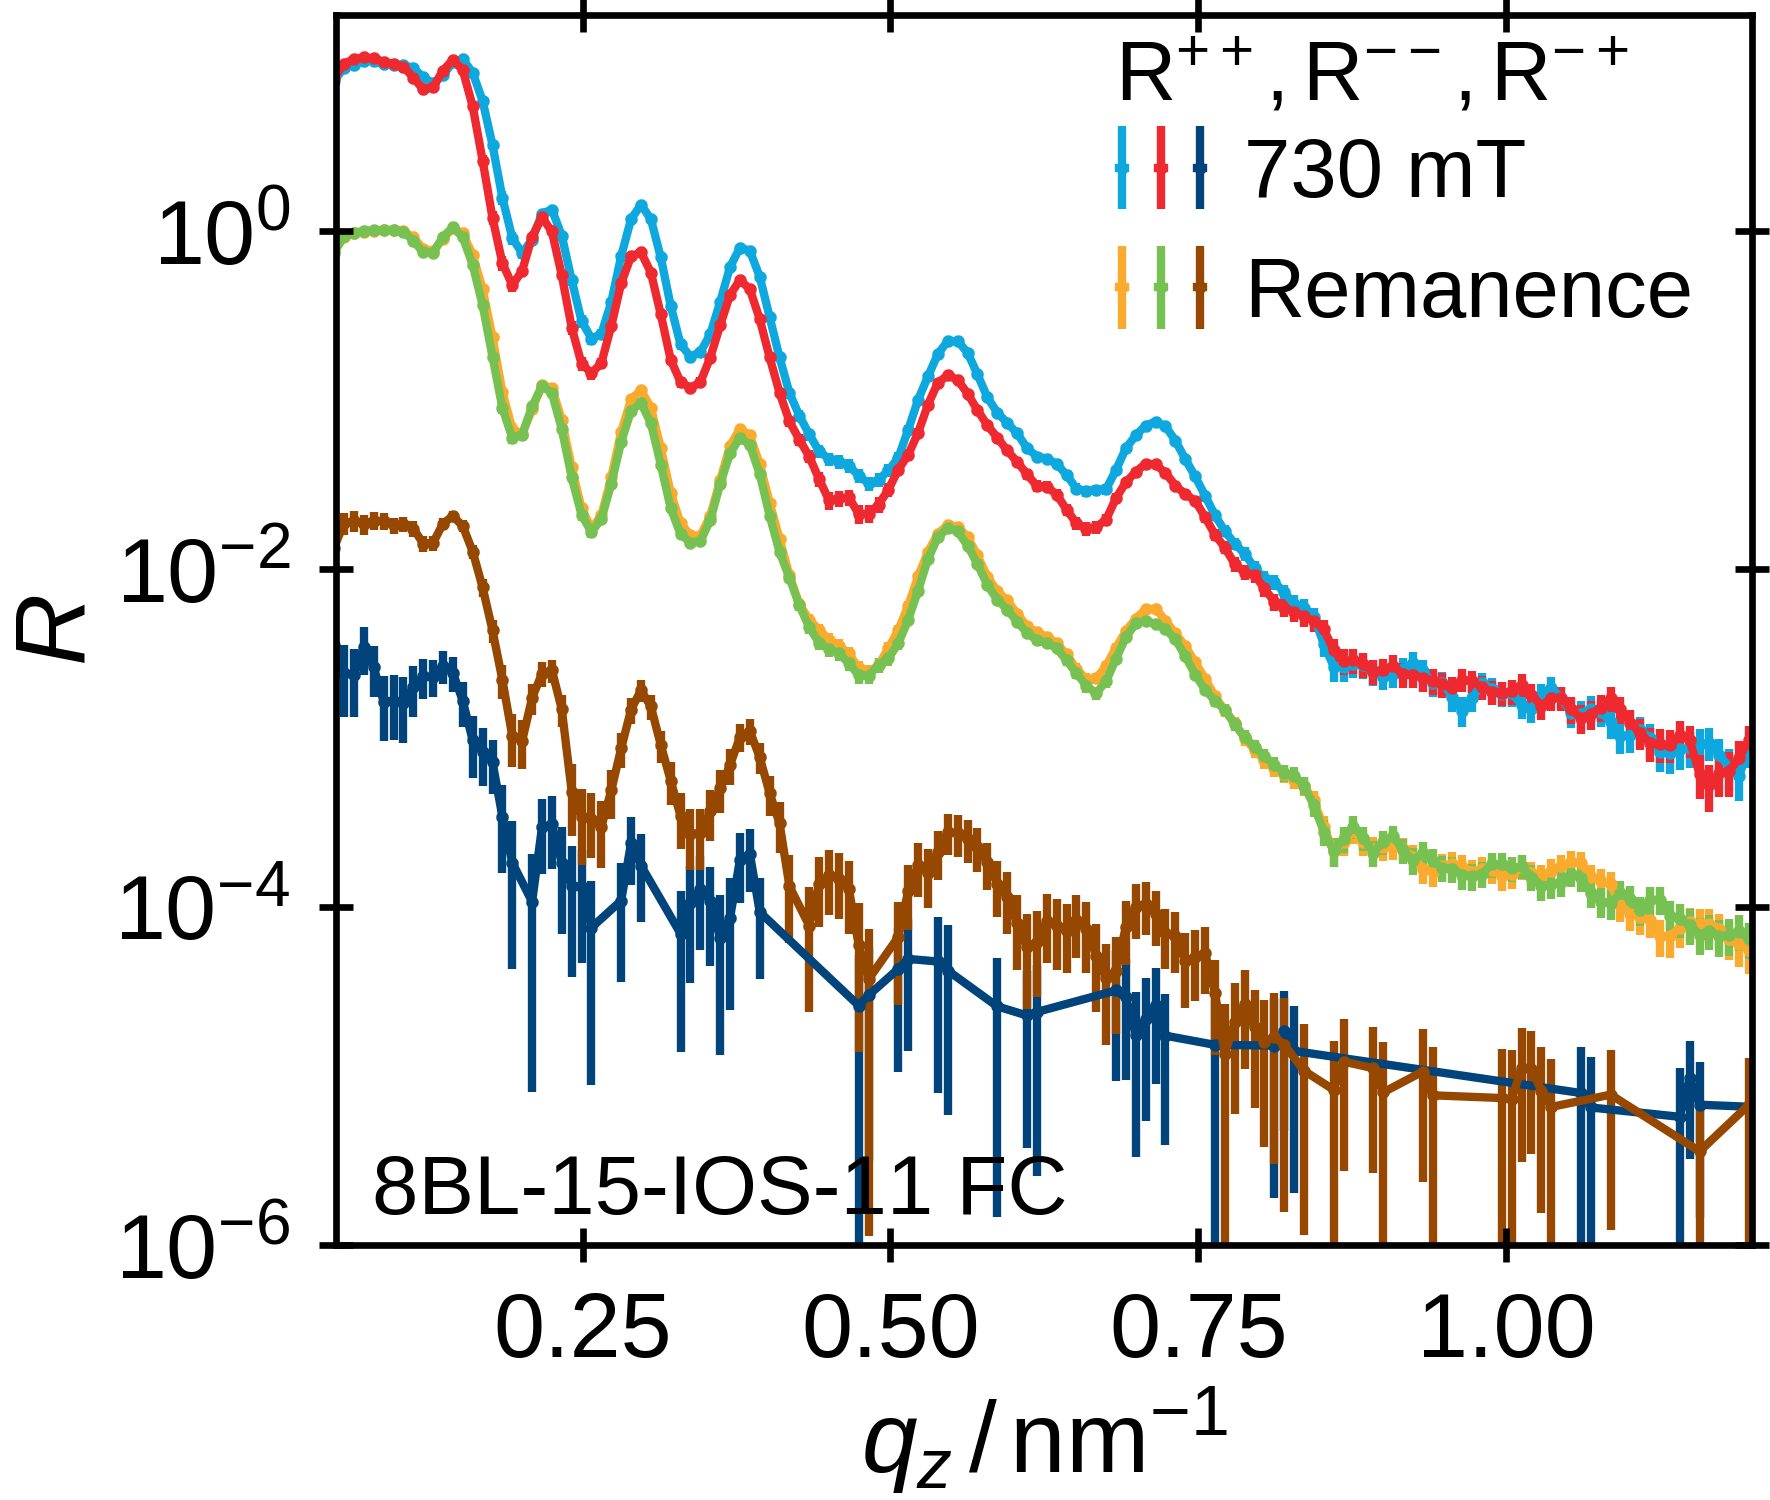
\includegraphics{looselyPackedNP_VerticalStructure_8BL-15-IOS-11_PNR_FC30K}
    \caption{\label{fig:looselyPackedNP:bilayer:pnr:8BL-15-IOS7}X-ray reflectometry from SC-IOS-11 (left) and SC-IOS-7 (right). The inset shows the scattering length density model of the fitted reflectometry curve (black).}
  \end{figure}

  \begin{figure}[tb]
    \centering
    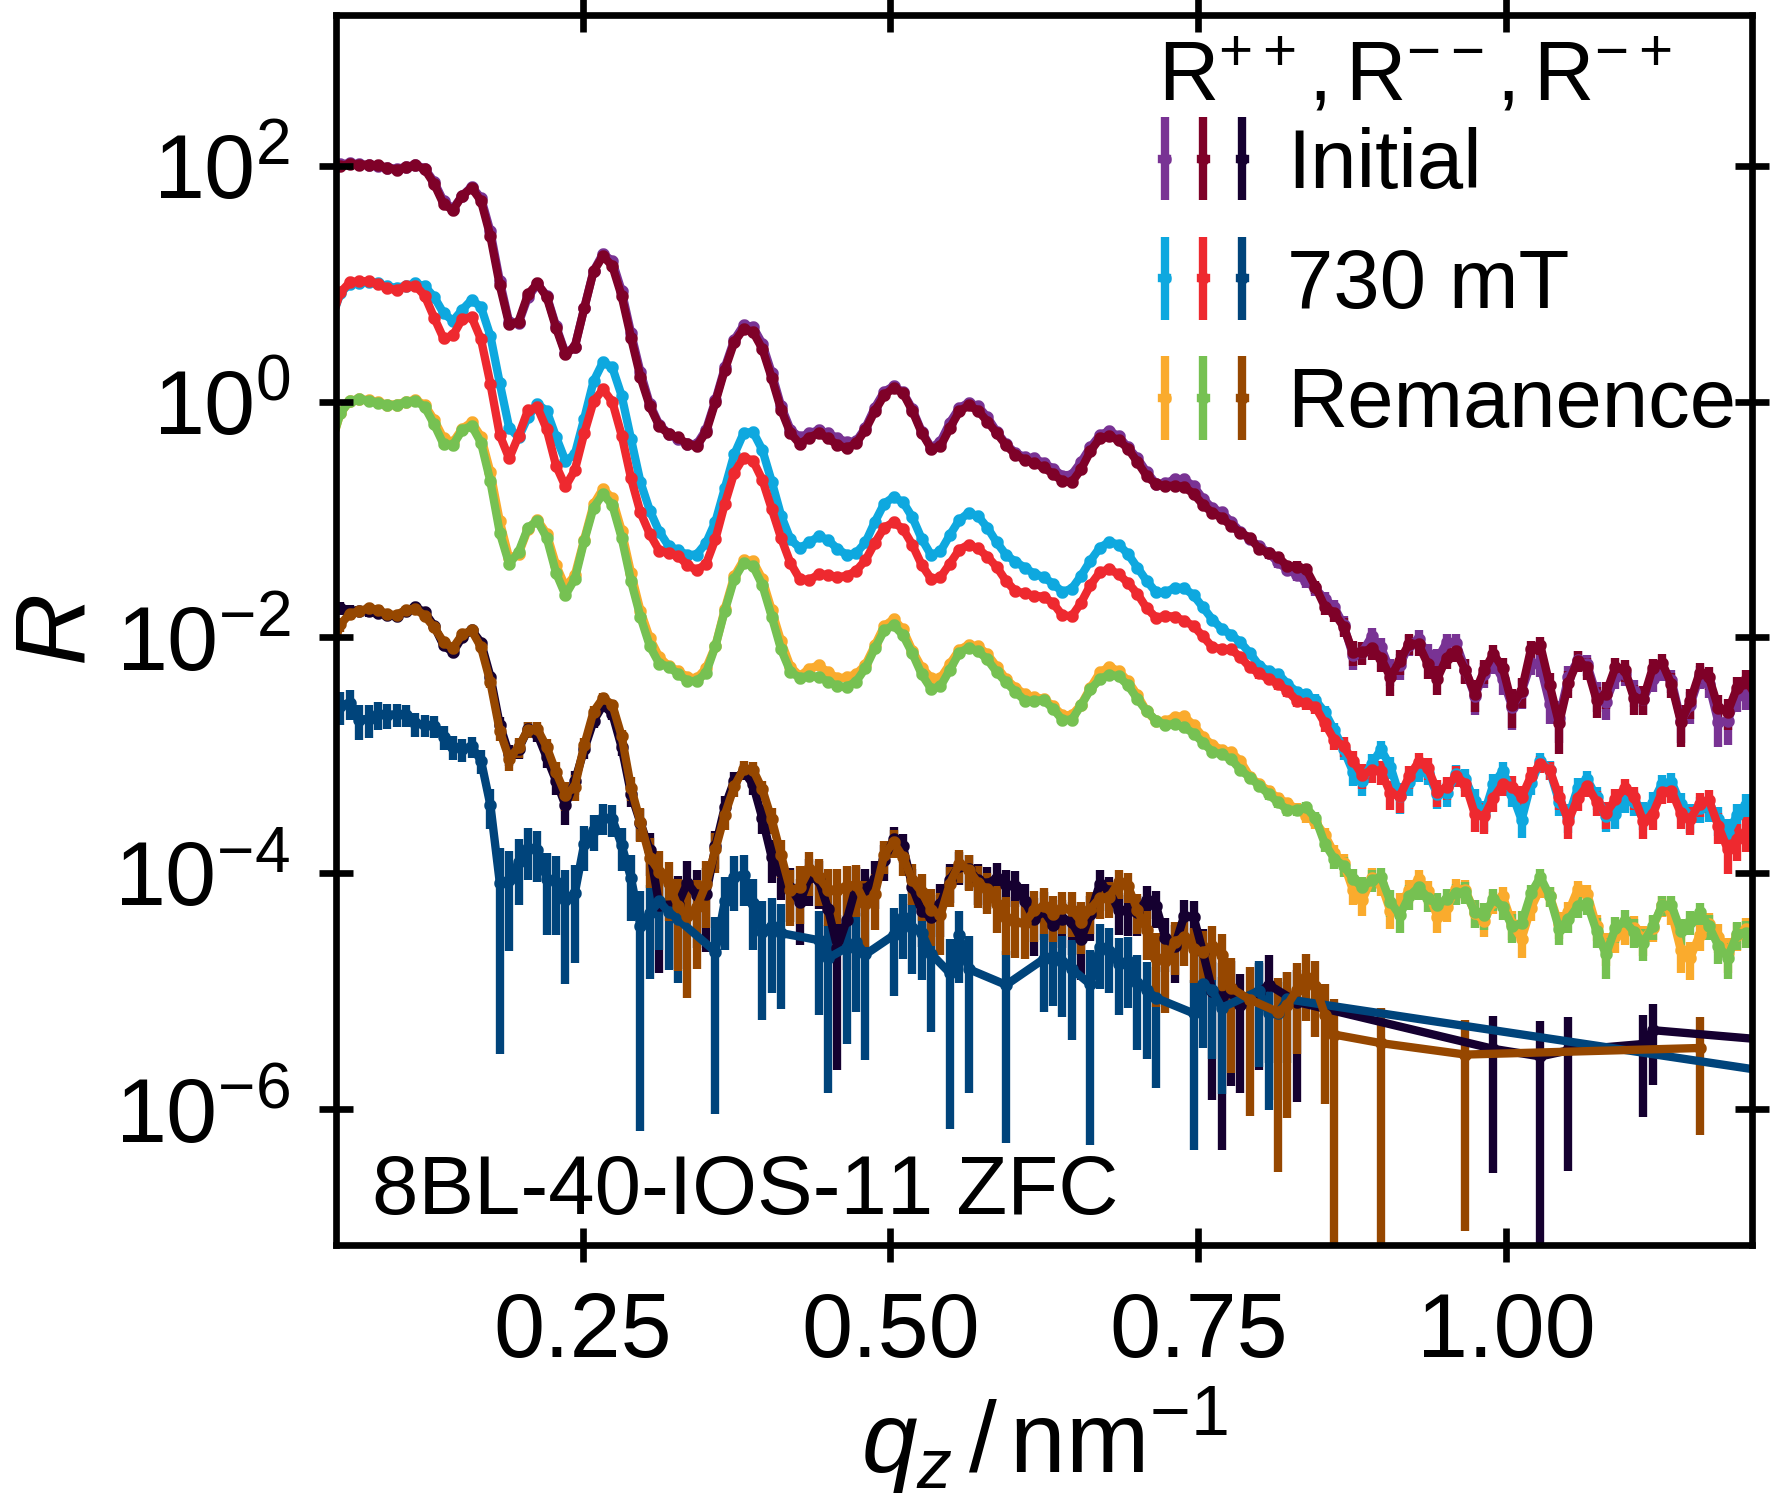
\includegraphics{looselyPackedNP_VerticalStructure_8BL-40-IOS-11_PNR_ZFC30K}
    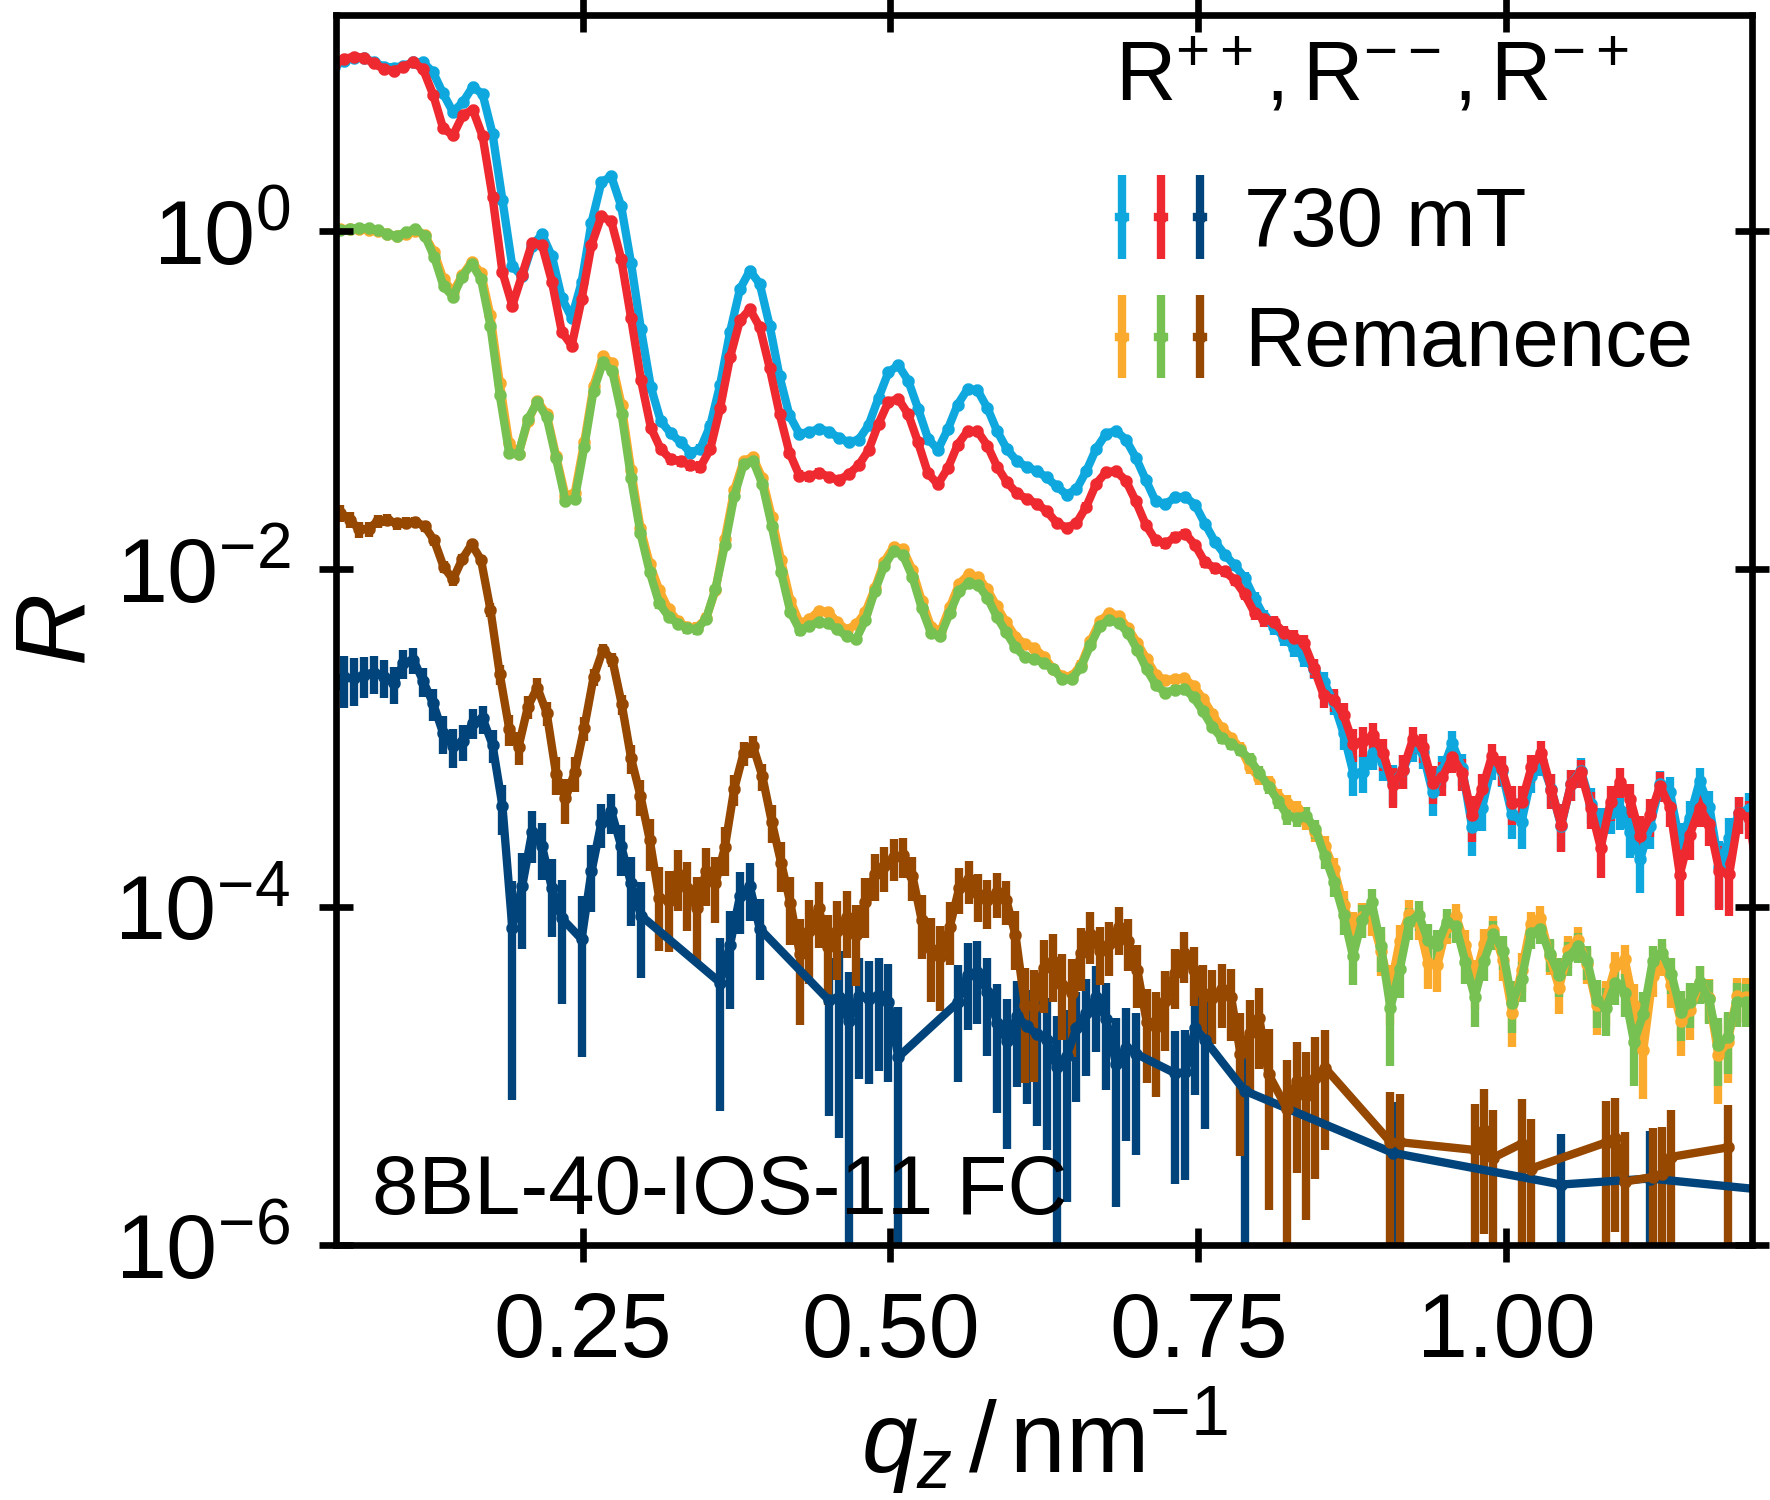
\includegraphics{looselyPackedNP_VerticalStructure_8BL-40-IOS-11_PNR_FC30K}
    \caption{\label{fig:looselyPackedNP:bilayer:pnr:8BL-15-IOS7}X-ray reflectometry from SC-IOS-11 (left) and SC-IOS-7 (right). The inset shows the scattering length density model of the fitted reflectometry curve (black).}
  \end{figure}

  Write about PNR

\end{document}